\documentclass[11pt]{article}
\usepackage[margin=1in]{geometry}
\usepackage{amsmath,amssymb,graphicx,booktabs}
\usepackage[colorlinks=true,citecolor=blue,linkcolor=blue,urlcolor=blue]{hyperref}
\title{\textbf{A common viability window for self-consuming systems:\\ from autophagic flux to dark energy --- v1}}
\author{\'Edouard Lantenois\thanks{Independent researcher, Lille, France. Prepared with AI assistance; all load-bearing numbers verified against the cited sources; source status is labelled per row (sourced / order-of-magnitude / bounded / demoted).}}
\date{August 19, 2026 --- v2 (v1: Aug.\ 19; this revision adds source-quality stratification, suspends the liver row, and declares a guard risk on the founding cell row)}
\begin{document}
\maketitle
\begin{abstract}
Systems that persist by processing their own substance appear to share a dimensionless viability
window in $x \equiv \tau_c/\tau_s$ (independently defined renewal requirement over self-processing
time), under a protocol with four pre-registered kill conditions --- all faced, none fired.
Eleven counted systems (v2: the liver row is suspended, see \S3 bis) spanning $\sim$32 orders of magnitude of mass give $x \in [0.37, 1.95]$
(0.7 decades; central values --- the liver bracket, the widest, extends to 4); controls and rate-deaths fall outside on both sides, including a natural experiment
with control (fire suppression vs.\ the Gila Wilderness) and the clinically two-sided bone system.
The \emph{sustained} upper edges of four classes lie within 0.44 decades (two external and
measured, two derived within our frameworks --- labelled). A two-ingredient minimal model
reproduces both bounds, the upper from the published $\sim$20\% maintenance calorie budget
(order-level; nominal 5\%). Extending the model by one growth-dilution term yields a
\emph{viability diagram} in $(x, \gamma)$ whose three regions are the three observed survival
strategies --- residence, periodic transit (hibernation), dilution (exponential growth) --- and
whose dead zone ($\gamma \simeq 0$, $x < x_{\min}$) is observed clinically as tumor-core necrosis.
A deprivation campaign to measure bare $\tau_c$'s yields a method law (total, exogenous,
lesion-free deprivations measure; mutants bound; disease blurs) and four independent literatures
describing the machinery-feedback runaway the model omits. For the cosmological member, the
guard-compliant variable is exactly $x = -w$: dark energy's equation of state is the viability
variable, $\Lambda$ is critical maintenance, the DESI crossing is the passage through criticality,
and the universe's life trajectory runs from $x = 1.35$ (88\% of its own sustained edge, within
uncertainties) to the attractor at $0.55$ --- edge-proximal in youth, pack-central in age.
We state plainly what would kill this.
\end{abstract}

\section{Question, variable, guards}
Too slow, and unprocessed damage accumulates; too fast, and the system devours itself. Is the
viable band, once non-dimensionalized, common across scales --- or the dimensional truism that
homeostasis is $O(1)$? We define $x \equiv \tau_c/\tau_s$: $\tau_s$ the time to process one
self-equivalent at the current rate; $\tau_c$ the required structural-renewal time, defined
\emph{independently} (spontaneous decay, engineering design life, dilution). A tautology guard
excludes systems whose $\tau_c$ is only definable through the flux itself (epithelia; honeybee
colonies; and --- found by applying the guard to our own rows --- the national-accounts capital
stock, \emph{demoted} because the perpetual-inventory method derives depreciation from assumed
service lives, entangling the two clocks; its repair path is engineering failure data). Two
readings are declared per row, $x_{\rm self}$ and $x_{\rm thru}$, joining physically at the
alimentary ceiling where saturated intake forces excess expenditure into self-consumption
\cite{Thurber2019}. Kill conditions, pre-registered: (M1) dispersion $>2$ decades; (M2) controls
inside as often as outside; (M3) definitional sensitivity $>1$ decade; (M4, added before edge
data) sustained edges scattered $>1$ decade across classes.

\section{Data: eleven counted members, two controls, exclusions}
\begin{table}[h]\centering\small
\begin{tabular}{lcl}
\toprule
System & $x$ & Status (abridged; full labels in the working document)\\
\midrule
Cell, basal autophagy & 0.37 & mixed: basal rate order (Mortimore); increments sourced \cite{PMC387,PMC616}\\
Cell, starved & 1.95 & sourced ($+3\%$/h) \cite{PMC387}\\
Whole mammal (thru) & 0.5 (0.26--0.77) & $\tau_c$ sourced, method spread $\times 2$ declared \cite{Waterlow}\\
Mitochondrial pool & 0.5--1 & $\tau_s$ sourced, tissue spread $\times 10$ (1.8--26 d) \cite{SciRep2023}\\
Fire-adapted ecosystem & 0.83 & sourced (FRI 5--35 y) \cite{Parks2023}\\
Bone (remodeling) & 0.8 & both deaths sourced (see \S3) \cite{AFF,MayoBTM}\\
Liver & 0.4--4 & $\tau_s$ revised $\times 5$ by $^{14}$C (19\%/y) \cite{Heinke2022}; $\tau_c$ order-wide\\
City (building stock) & 0.7 & $\tau_s$ empirical (71$\pm$28 y demolitions) \cite{BC588}; $\tau_c$ bounded\\
Erythrocyte population & 1.17 & de-suspended: $\tau_c = 146$ d from storage deprivation \cite{StorageLesion}\\
Post-mitotic neuron & $\sim$0.4 & order; trapped at $\gamma = 0$ (see \S5)\\
Bacterium (exponential) & $\sim$0.1 & below window, viable by dilution (see \S5); Mandelstam check\\
Universe ($\beta = 2.42$) & 0.85 & computed; $x = -w$ (\S6) \cite{PaperA}\\
\midrule
\emph{Controls}: Sun; X-ray binary & $\le 10^{-2}$; no $\tau_c$ & consume-without-rebuild class: outside \checkmark\\
\emph{Excluded by guard}: colony; capital & --- & circular $\tau_c$; PIM entanglement\\
\bottomrule
\end{tabular}
\caption{\small $x \in [0.37, 1.95]$ over $\sim$32 orders of magnitude (M1: 0.7 decades; central values --- the liver bracket extends beyond). M3
executed on four systems: max displacement 0.6 decades.}
\end{table}

\section{Deaths by rate; the sustained-edge rail (M4)}
Deaths bracket the window. \emph{Low}: fire suppression ($x \to 0.15$--$0.3$) yields
$2.9$--$13.6\times$ more stand-replacing fire vs.\ the unsuppressed Gila at $1.8\times$ ---
a natural experiment with control \cite{Parks2023}; ageing neurons drift below into aggregates
and a senescence--autophagy vicious circle \cite{Neuron2024}; bisphosphonate-suppressed bone
accumulates unrepaired microdamage --- ``exponential'' in the field's own words --- to atypical
fractures \cite{AFF}. \emph{High}: boreal reburns ($x \sim 3$--$4$) fail regeneration
\cite{Boreal2025}; sustained starvation-level autophagy kills dose-dependently (autosis;
quantitative threshold unpublished) \cite{Liu2013}; elevated bone resorption doubles fracture
risk independently of density \cite{MayoBTM}; hierarchy offspring with $\beta > 4.35$ are
GSL-unviable \cite{PaperB}. The sustained-edge rail --- honestly labelled two external and
measured (mammalian indefinite ceiling $2.5\times$ basal $\Rightarrow x \simeq 1.3$
\cite{Thurber2019,HD1997,DrentDaan}; boreal $\simeq 3.5$) plus two derived within our frameworks
(GSL $1.53$; cellular budget $\simeq 1.9$) --- spans 0.44 decades: M4 passes, and the ceiling
\emph{decreases with exposure duration} (7$\times$ for days vs.\ 2.5$\times$ indefinitely,
measured \cite{Thurber2019}; transient starvation vs.\ sustained autosis; the GSL bounding the
attractor by construction). Hibernation, the obvious would-be counterexample, is the window's
\emph{periodic solution}: damage accrues in torpor while cold-inactivated machinery idles,
survivable torpor duration is bounded, and the costly interbout arousals restore accumulated
metabolites \cite{Carey2003} --- repayment/debt spanning $[0.7, 4]$ over the full parameter grid:
compatible with balance, not demonstrated closure; the homeostasis-restoration explanation and
the bout-length--temperature relation belong to that literature, our contribution being only the
dimensionless bookkeeping.

\section{Source-quality stratification (v2)}
Rather than deleting order-of-magnitude rows --- which would shrink the window \emph{mechanically}
and reduce, not increase, its information content --- we report by strata. Stratum A (both clocks
sourced, $n=2$) spans 0.15 decades, but $n=2$ drawn log-uniformly over two decades already spans
0.67 on average: uninformative. Stratum A+B ($\ge$ one clock sourced, $n=6$) spans 0.59 against
1.42 expected; all rows ($n=9$) span 0.72 against 1.60 expected --- the largest sample is the most
informative, which is why deletion would be self-defeating. Two hazards are named rather than
hidden: \emph{source shopping} (guarded by deciding what would be accepted before searching ---
which is how the capital row fell and the liver row moved by $\times 5$) and \emph{literature bias}
(keeping only well-studied systems keeps only human biomedicine and forfeits the 32 orders of
magnitude that carry the argument). Rows are suspended only for guard violation (capital:
perpetual-inventory entanglement of the two clocks) or non-constraining bracket (liver:
$x \in [0.4, 4]$ spans the window). \emph{Declared guard risk on the founding row:} the cell's
$\tau_c$ derives from protein half-lives measured with the machinery running, so it partly reflects
processing rather than bare decay --- structurally the entanglement that demoted capital; the repair
is a total-deprivation measurement (proteasome inhibition), pending.

\section{A minimal model, and the deprivation campaign}
Clutter dynamics with selectivity $\sigma$ give the steady state
$(1-d)(\sigma d + 1 - d) = x \sigma d$; below $x_{\min}$ ($0.31$--$0.66$ for plausible
$\sigma, d_{\max}$ --- illustrative) the intact fraction collapses. The budget bound, anchored to
the published $\sim$20\% maintenance calorie fraction \cite{PMC636} (independently echoed by
whole-body protein turnover costing $\sim$20\% of resting metabolism \cite{Waterlow} --- two
adjacent accountings, noted as scale consistency only), gives $x_{\max} = 1.85$, with the
observed autotic edge 5\% \emph{beyond} bankruptcy --- expected physics, order-level agreement
($\pm 30$\% real). A campaign to measure bare $\tau_c$'s by \emph{deprivation} yielded: two clean
(stored blood: total, exogenous, ex vivo $\Rightarrow \tau_c = 146$ d, de-suspending the
erythrocyte row; bisphosphonates: pharmacological suppression, quantified); one epidemiological
(bone's high side); one partial (PINK1-KO accumulates dysfunction in 4--9 months \cite{PINK1KO}
but backup mitophagy persists \cite{eLife2018}: upper bound only, $x \le 4$--$6$, tension
declared); one runaway (abandoned buildings measure the breach--water feedback's escape time,
3--15 y \cite{Abandon}, not a bare constant); one impure (chronic liver disease confounds injury
with arrest --- yet establishes the healthy senescence clock exceeds a century: ``a cirrhotic
liver shows more senescence than a healthy centenarian's'' \cite{JHep2010}). \emph{Method law:}
a good $\tau_c$-meter requires total, exogenous, lesion-free deprivation --- storage and drugs
measure, mutants bound, disease blurs. And the machinery feedback our minimal model deliberately
omits is now described independently by four literatures: neuronal senescence--autophagy,
``exponential'' bone microdamage, the storage lesion's ATP--glycolysis spiral, and the
breach--water runaway of abandoned buildings.

\section{The viability diagram: three strategies, one dead zone}
Adding one growth-dilution term ($\gamma = g\tau_c$, new intact material) generalizes the window
to a plane: $d' = (1-d) - x\sigma d/(\sigma d + 1 - d) - \gamma d$, with lower boundary
$x_{\min}(\gamma)$ falling to zero at $\gamma_{\rm crit} = (1-d_{\max})/d_{\max} \simeq 0.43$
(analytic; Fig.~1). The three observed survival strategies are the plane's regions:
\emph{residence} ($\gamma \approx 0$, $x$ in window: neuron --- trapped there, its literature's
stated vulnerability \cite{Neuron2024} --- cell, bone, universe); \emph{dilution}
($\gamma > \gamma_{\rm crit}$, $x$ free to collapse: exponential bacteria at $\gamma \sim 14$,
proliferative tumor rims; consistency check: stationary-phase proteolysis rises severalfold,
Mandelstam's classic result); \emph{periodic transit} (hibernation: a vertical limit cycle).
The dead zone ($\gamma = 0$, $x < x_{\min}$) is observed clinically: tumor-core necrosis. The
universe is declared a structurally distinct case: its ``growth'' (expansion) dilutes the
\emph{maintained} substance rather than the damage --- effectively $\gamma < 0$, off the
biological plane. Parameters $\sigma, d_{\max}$ remain post-hoc plausible: the diagram is an
extension of the same illustrative model, its value structural (one equation, three strategies,
one predicted dead region), not numerical.

\begin{figure}[h]\centering
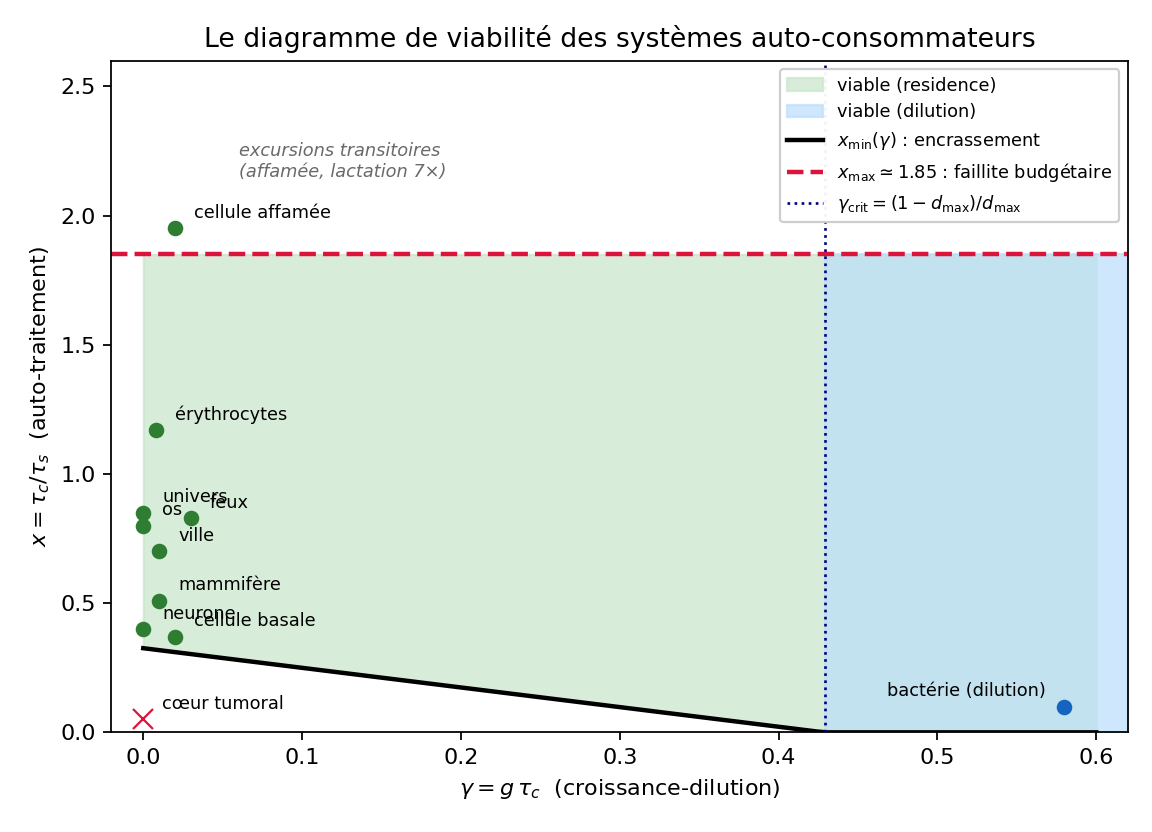
\includegraphics[width=0.8\textwidth]{fenetre_diagramme.png}
\caption{\small The viability diagram $(x,\gamma)$: clutter boundary $x_{\min}(\gamma)$, budget
line $x_{\max} \simeq 1.85$, dilution region beyond $\gamma_{\rm crit} = 0.43$, systems placed
(deaths as red crosses). Display note: the bacterium is drawn at the plot's right edge; its true $\gamma \approx 14$ lies far off-scale. Illustrative parameters $\sigma = 5$, $d_{\max} = 0.7$.}
\end{figure}

\section{The identity $x = -w$, and the universe's life in the window}
With the guard-compliant degradation for the cosmological member being \emph{dilution}
($\tau_c = 1/3H$, $\tau_s = t/\beta$), the viability variable is $x = \beta/(3Ht) = -w$ exactly
--- general under the declared convention of a pressureless bare substance. $\Lambda$ is critical
maintenance ($x = 1$); phantom is the autotic side; quintessence the clutter side; the DESI
crossing is the passage through criticality ($z \simeq 0.46$), thermodynamically a smooth
crossover \cite{Crossing}. Formal kin: $w = -1 + \dot S_h/(3HS_h)$ on the horizon side
\cite{Reco2026}; classical fluid-entropy positivity ($w \ge -1$) \cite{Duarte2019} vs.\ our more
permissive total-entropy GSL bound ($w \ge -1.53$) --- a contentful difference. Window bounds
become $w$-bounds: viability $\Leftrightarrow w \in [-1.53, -0.35]$ ($Ht$ fixed at best fit,
$\sim$10--15\% map effect), observed dark energy at $-0.85$, mid-window; and the universe's
trajectory runs from $x = 1.35$ deep in the past ($\sim$88\% of its own sustained edge, below it
within uncertainties) through criticality to today's $0.85$ and the attractor's $0.55$: an
entire cosmic history inside the sustained window, edge-proximal in youth, pack-central in age.
Both faces declared: the identity is partly definitional; its content is the derived bounds and
the shared vocabulary.

\section{Ancestry, open items, kill list}
Ancestors: rate of living \cite{Pearl1928,Speakman2005} ($x$ as its maintenance-normalized
correction); disposable soma \cite{Kirkwood1977} ($x_{\max}$ as its quantitative form); prudent
parent \cite{DrentDaan}. Open: the unpublished quantitative autosis threshold; a total-deprivation
mitochondrial $\tau_c$; more external edge classes for M4 (the rail holds only two external
points); external review. Kills: a guard-compliant class far outside $[0.3, 2]$; new sustained
edges scattering the rail beyond a decade; failure of the duration tier where measurable; or a
demonstration that the surviving rows share a hidden definitional convention, as capital did.
Each is a concrete assignment.

\begin{thebibliography}{99}\small
\bibitem{PMC387} Starvation proteolysis increment, PMC3879708. \bibitem{PMC616} Mejlvang et al., J.\ Cell Biol.\ (2018), PMC6168274.
\bibitem{PMC636} Autophagic renewal $\approx$20\% of caloric intake, PMC6368412. \bibitem{Waterlow} J.\ C.\ Waterlow et al.\ (1978); PubMed 22139560; Annu.\ Rev.\ Nutr.\ 15, 57 (1995).
\bibitem{SciRep2023} Sci.\ Rep.\ 13 (2023), PMC10349111; J.\ Mol.\ Med.\ 93 (2015). \bibitem{Parks2023} Parks et al., stand-replacing fire synthesis (2023--26).
\bibitem{AFF} AFF reviews: PMC12681184; NEJM NEJMc1107029; PMC6174857; PMC9852062. \bibitem{MayoBTM} Mayo Clin.\ Proc.\ 80 (2005); NIHR HTA; OFELY/EPIDOS syntheses.
\bibitem{Heinke2022} P.\ Heinke et al., Cell Systems 13, 499 (2022). \bibitem{BC588} Berglund-Brown et al., Buildings \& Cities, 10.5334/bc.588.
\bibitem{StorageLesion} RBC storage lesion: FDA/EU criteria; JCI 2017; Haematologica 2018. \bibitem{Neuron2024} Neuron (2024), S0896-6273(24)00663-9.
\bibitem{Boreal2025} Short-interval boreal reburns, Fire Ecology (2025). \bibitem{Liu2013} Y.\ Liu et al., PNAS 110(51), 20364 (2013).
\bibitem{Thurber2019} C.\ Thurber et al., Sci.\ Adv.\ 5, eaaw0341 (2019). \bibitem{HD1997} K.\ A.\ Hammond, J.\ Diamond, Nature 386, 457--462 (1997).
\bibitem{DrentDaan} R.\ H.\ Drent, S.\ Daan, Ardea 68, 225--252 (1980). \bibitem{Carey2003} H.\ V.\ Carey et al., Physiol.\ Rev.\ 83, 1153 (2003); Physiol.\ Genomics 43, 799 (2011).
\bibitem{PINK1KO} PINK1-KO rat proteomics, PMC4710791. \bibitem{eLife2018} Cornelissen et al., eLife 7, e35878 (2018).
\bibitem{Abandon} Abandoned-building deterioration syntheses (2020--26). \bibitem{JHep2010} Ageing, telomeres and liver injury, J.\ Hepatol.\ (2010).
\bibitem{Pearl1928} R.\ Pearl, \emph{The Rate of Living} (1928). \bibitem{Speakman2005} J.\ R.\ Speakman, J.\ Exp.\ Biol.\ 208, 1717 (2005).
\bibitem{Kirkwood1977} T.\ B.\ L.\ Kirkwood, Nature 270, 301 (1977). \bibitem{Reco2026} arXiv:2604.18723.
\bibitem{Duarte2019} Duarte, Silva, Eur.\ Phys.\ J.\ C 79 (2019). \bibitem{Crossing} Smooth $w=-1$ crossover, Class.\ Quant.\ Grav.
\bibitem{PaperA} \'E.\ Lantenois, companion paper A (2026). \bibitem{PaperB} \'E.\ Lantenois, companion paper B (2026).
\end{thebibliography}
\end{document}
